\section{Gazebo}
\label{sec:gazebo}

Gazebo \citep{cit:koenig2004} merupakan sebuah simulator robot bersifat \emph{open source} yang dapat digunakan untuk mensimulasikan model robot secara virtual di lingkungan 3D.
Awalnya, Gazebo merupakan bagian dari Player Project \citep{cit:gerkey2003} yang memungkinkan sebuah simulasi robot 2D (Stage) dan 3D (Gazebo) dapat bekerja dengan sebuah program yang dibuat secara terabstraksi untuk robot (Player).

Untuk memungkinkan sebuah simulator robot dapat bekerja,
  Gazebo mengintegrasikan ODE dan Bullet sebagai physics engine,
  OpenGL untuk rendering model dan lingkungan,
  serta beberapa program lain untuk mensimulasikan sensor dan aktuator secara virtual.
Gazebo memiliki berbagai macam sensor dan aktuator virtual yang dapat digunakan di lingkungan simulasi seperti sensor kamera, motor, \emph{lidar}, IMU, dan lain sebagainya.

\begin{figure}[ht]
  \centering
  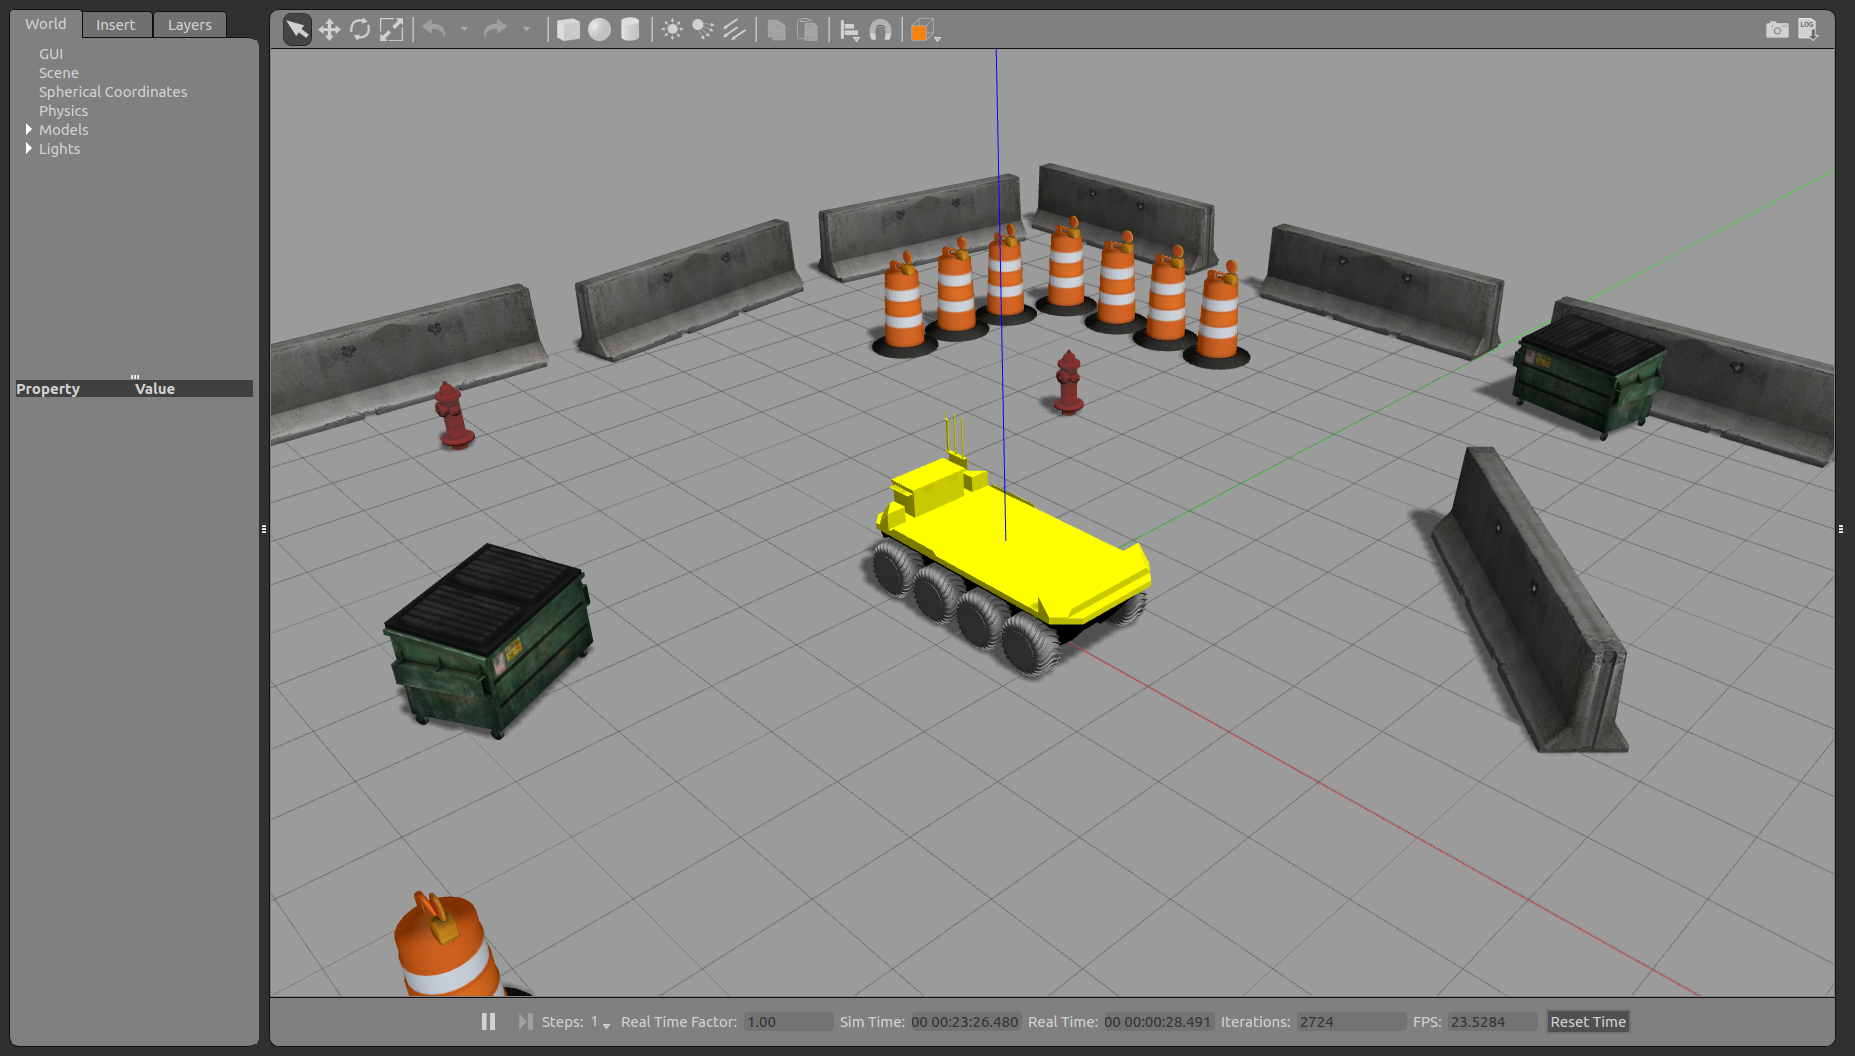
\includegraphics[width=0.95\textwidth,keepaspectratio]{gambar/contoh-gui-gazebo.png}
  \caption{Contoh tampilan GUI dari simulator Gazebo \citep{url:gazeboexample}.}
  \label{fig:contohguigazebo}
\end{figure}

Pada Gazebo, keseluruhan sistem yang ada di simulasi akan dijalankan secara \emph{headless} menggunakan program \lstinline{gzserver}.
Selain itu, seperti yang terlihat pada gambar \ref{fig:contohguigazebo},
  Gazebo juga menyediakan \emph{gzclient}, sebuah program GUI yang memungkinkan pengguna untuk melihat tampilan dan memanipulasi model maupun lingkungan simulasi yang sedang berjalan di simulator.

\subimport{3-gazebo}{1-gazebo-model.tex}
\subimport{3-gazebo}{2-gazebo-plugins.tex}
